%%%%%%%%%%%%%%%%%%%%%%%%%%%%%%%%%%%%%%%%%%%%%%%%%%%%%%%%%%%%%%%%%%%%%%%%%%%%%
%
% This file is delivered as an usage example of the file 'kkr13-eng.sty'.
% The style file 'kkr13-eng.sty' has been prepared for papers intended 
% to be presented at the XIII National Conference on Robotics in Poland.
%
% The file 'kkr13-eng.sty' contains definitions of macros for English
% and Polish authors. Thus their names are in English and Polish respectively.
% They define the same operations. English and Polish names are used
% only for authors' convenience. 
% Therefore both types of macros can be used in this type of the document.
% The same type of macros are defined in the style file defined for papers 
% written in Polish.
% Below there is a list of macros names in English and their equivalent forms
% in Polish.
%
%       \articleTitle          =   \tytulArtykulu
%       \titleFootNote         =   \stopkaPrzypisTytulu
%       \articleAuthor         =   \autorArtykulu
%       \affiliation           =   \instytucja
%       \theSameAffiliationAs  =   \instytucjaTaSamaJak
%       \articleShortTitle     =   \naglowekTytulSkrocony
%       \breakAuthorsLine      =   \zlamLinieAutorow
%       \authorsForHeader      =   \naglowekAutorzyArtykulu
%       \authorsCustomizedList =   \wlasnaListaAutorow
%       \abstract              =   \streszczenie
%       \Equation              =   \wzor
%       \refeq                 =   \refwzor
%       \reffig                =   \refrys
%       \refFig                =   \refRys
%
% Author: Bogdan Kreczmer 
% Last modification:      2013.12.09
% 
% In the case of any doubt, please, contact via e-mail.
% The address of the author is:
%  bogdan.kreczmer@pwr.wroc.pl
%
%%%%%%%%%%%%%%%%%%%%%%%%%%%%%%%%%%%%%%%%%%%%%%%%%%%%%%%%%%%%%%%%%%%%%%%%%%%%



\documentclass[11pt,twoside]{article}
\usepackage{kkr13-eng}
\usepackage{todonotes}
\usepackage[hidelinks]{hyperref}
\usepackage{array}
\usepackage{booktabs}
\usepackage{cite}
\newcommand{\superscript}[1]{\ensuremath{^{\textrm{#1}}}}
\newcommand{\subscript}[1]{\ensuremath{_{\textrm{#1}}}}

\articleTitle{3D Object Classification \\ Based on RGBD Images}

%
% For information of a project (if any)
%
\titleFootNote{The work described in this paper was conducted within author's Bachelor's dissertation}

%
% Parameters:
%   1 - initials of the first and middle name of an author
%   2 - the first and middle name of an author
%   3 - the last name of an author
%
\articleAuthor{A.}{Adam}{Kosiorek}

\affiliation[institute1]{ Institute of Automation and Robotics, The Faculty of Mechatronics of Warsaw University of\\ Technology, email: iair@mchtr.pw.edu.pl, website: http://iair.mchtr.pw.edu.pl}

\bibliographystyle{abbrv}
\begin{document}


%\listoftodos

\abstract{ 

  This paper introduces a Bag of Words (BoW) semantic object classification framework based on RGBD data registered by a Microsoft Kinect camera. The BoW concept in natural language processing is introduced and a BoW image processing pipeline is described. Each part of the pipeline (region detection, feature extraction and vector quantization) is characterized and the most successful algorithms are outlined. Applications of BoW in image processing and their results are discussed. Additionally, the problem of classification is described. Algorithms with high performance potential were identified and evaluated. Salient region detection is done by SIFT, ISS3D and Uniform Sampling. Description is performed by FPFH, PFH and PFHRGB. Vector quantization was carried out by the KMeans algorithm. An SVM with the RBF kernel trained with an All-vs-All was used as a classifier. We achieved the accuracy of 65.22\% on 8 categories of the Berkely 3D Object Dataset and 62.3\% on a 10 category dataset compiled by Zhang from the Tokyo University.
}

\maketitle

\section{ INTRODUCTION }

  It has never been easier to capture visual information. Popular storage services grow lighting fast due to terabytes of photographs and movies uploaded every day. The growth is so fast that hand-tagging and description, the traditional means of annotation, cease to suffice. They are ambiguous, emotional and rarely optimal. With no better solution at hand databases are becoming increasingly harder to browse. Another, but quite similar setting occurs in the field of mobile robotics. A mobile robot is there to interact with its environment. If so, it would be desirable for the robot to know what kind of surroundings it is in. The problem can be treated as a scene or object classification problem, one of the most popular computer vision issues in the last decade \cite{ponce2011cv}. 

  This paper tackles two issues. Firstly, the Bag of Words (or BoW for short) approach to image classification is reviewed. The Bag of Words method originated from the natural language processing domain \cite{tsai2012bag}. It makes a strong assumption that word occurrence in a text document define its meaning. It were Csurka \textit{et al} who first used BoW for image classification in 2004 \cite{csurka2004visual}. Since images cannot be simply cast into natural language documents a pipeline that help us achieve this goal is needed. It usually consist of: keypoint detection, feature extraction, vector quantization together with codebook construction and classification, steps that will be discussed later.

  Being efficient, effective and flexible, a Bag of Words processing pipeline is, however, a blessing in a disguise. While in fact it can provide satisfactory results with little effort, it is cumbersome to tune, thus spectacular performance is hard to achieve. One reason is the abundance of suitable algorithms available. Wide variety of building blocks might make it flexible, but it renders choosing an optimal combination infeasible.

  The rest of this work is organised as follows: Section 2 describes the Bag of Words technique in detail. Construction of an image model is discussed and the most popular algorithms are outlined. Then, applications of BoW in computer vision are reported and the problem of classification is introduced. Section 3 describes two renown RGBD image datasets suitable for evaluation of RGBD data-based object classifiers. Section 4 addresses the topics of experimental setup, conducted experiments and provides the results. Finally, Section 5 concludes this work.

\section{ BAG OF WORDS }

  The Bag of Words model is an intermediate representation in a form of a histogram used in natural language processing, information retrieval and data mining. It obliterates any grammatical information as well as word order so as to preserve word incidence only.

  \begin{figure}[!ht]
  \centering
  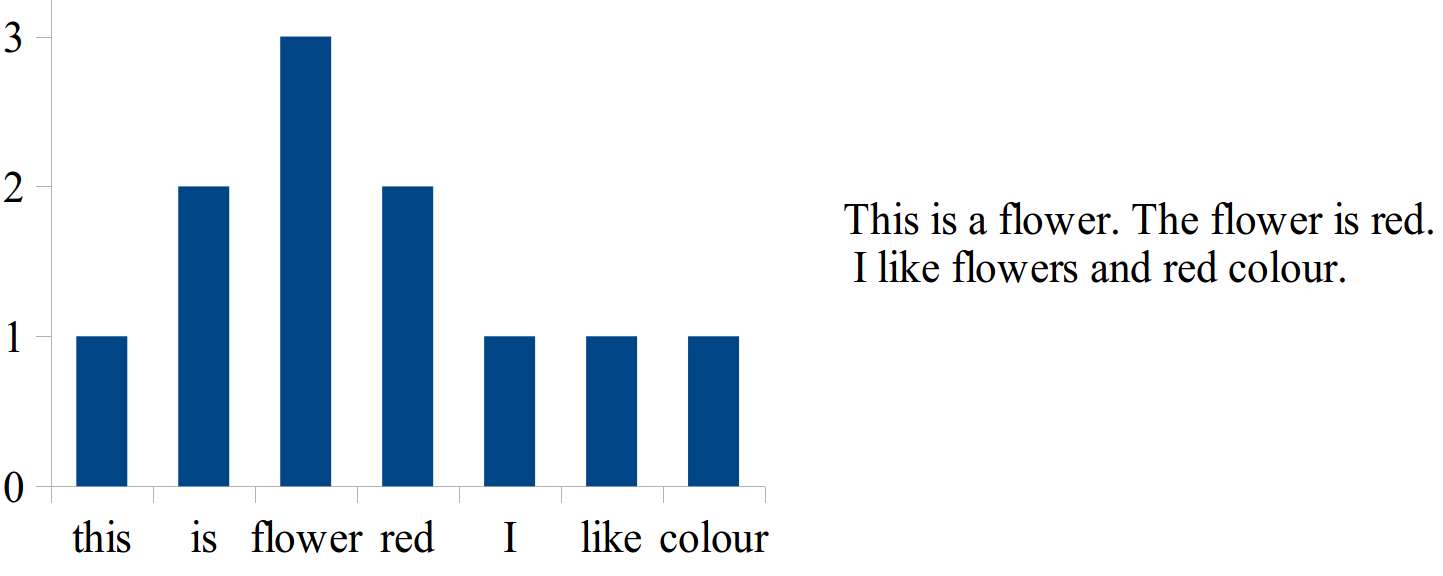
\includegraphics[width=0.7\textwidth]{../figs/bow_example}
  \caption{Bag of Words histogram}
  \label{fig:bow_example}
  \end{figure}

  \refFig{fig:bow_example} shows a piece of text and its BoW model, with articles and punctuation marks left out. In order to compare different documents a global dictionary (codebook) must be built. It is constructed by taking every unique word from all available documents. One can image that if a dictionary is of any considerable size the resulting representation of especially small documents can be very sparse. Classification algorithms can be optimised for sparse data in order to boost performance.

  In natural language processing BoW is used to infer semantic meaning of documents. If we could translate an image into a text document we might be able to employ similar methods. A question arises: How does one make a text document from an image?

  \subsection{Processing Pipeline}	
    Tsai describes a well established pipeline that allows translation of images into text documents \cite{tsai2012bag}. It consists of the following steps: (1) region detection, (2) feature extraction, (3) vector quantization and (4) BoW histogram formation as can be seen in \refFig{fig:bow_pipeline}. The author summarises the most commonly used methods for performing these tasks. 

    \begin{figure}[!ht]
    \centering
    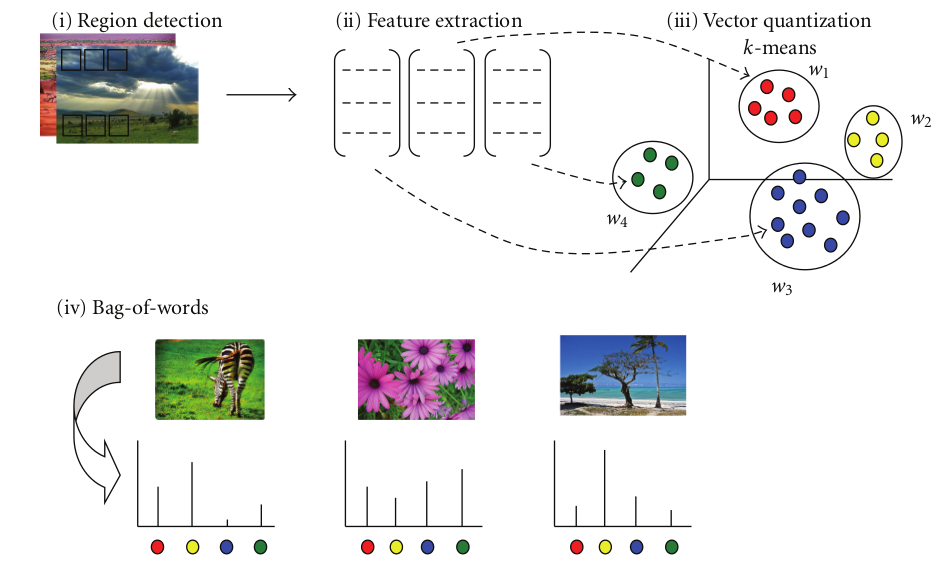
\includegraphics[width=0.75\textwidth]{../figs/tsai2012}
    \caption{Bag of Words pipeline. The figure comes from \cite{tsai2012bag}}
    \label{fig:bow_pipeline}
    \end{figure}
	
  \subsubsection{Region Detection}
    Characteristic region detection is the first step in any Bag of Words framework. Numerous detection methods have been developed, which might choosing the right one tricky. The most common detectors use a Harris corner detector or 1\textsuperscript{st} or 2\textsuperscript{nd} image derivatives. A Harris-Laplace detector is an example of a Harris-based detector. The Harris function is scale adapted and its outcome is subjected to a Laplacian-of-Gaussian (LoG) operator, which selects points in scale space. 2\textsuperscript{nd} image derivatives~---~Hessians can be combined with a LoG operator in order to further select points in the Hessian's determinant space.

    A number of more advanced recipes for salient region localisation have been developed and implemented. These include for example SIFT \cite{sift_keypoint}, SUSAN \cite{susan_keypoint} and ISS \cite{iss_keypoint}, with the vast majority implemented for the 2D domain and only a few generalised to 3D. A comparative study of detectors available in the PointCloud Library (PCL) can be found in \cite{pcl_keypoint_comparision, 3d_keypoint_eval}. All of the above, called sparse feature detectors, resort to selection of maxima in specific state spaces. An entirely different scheme is to use a dense feature detector, that is to take a uniformly sampled grid of points. Dense detectors are advantageous in that they sample slow changing regions in terms of image derivatives. Examples of such regions are a clear sky or a calm ocean. Li \emph{et al} showed that dense detectors generally outperform sparse ones \cite{fei2005bayesian}.
    
  \subsubsection{Feature Extraction}
    Suppose only keypoint's coordinates were given. The smallest affine transformation applied to the image would render the keypoints useless. Feature extraction is about describing a region in a way that is invariant to affine transformations, light intensity changes or colour saturation. Achieving all these properties simultaneously can be hard but methods that achieve some of them do exist. Keypoint description takes form of coordinates in a high-dimensional space. One of the most precise and repeatable algorithm is SIFT \cite{sift_features}, which is a 3D histogram of gradients structured as a 128-dimensional vector of floating point values. It is the most often extracted descriptor in BoW pipelines. Other methods include various colour descriptors, binary descriptors such as 512-dimensional GIST \cite{ponce2011cv}. There are techniques designed for 3D exclusively. Among them are Persistent Point Feature Histogram (PFH) \cite{pfh_rusu2008}, its faster alternative FPFH \cite{fpfh_rusu2009} and PFHRGB, which takes into account colour information, all implemented in PCL.
    
  \subsubsection{Vector Quantization}
    Vector quantization comprises of: (1)~codebook construction from a trainset and (2)~descriptor parsing, performed on a test set only on all data, depending on the setting. The simplest way of building a dictionary is to find patterns or regions within descriptors computed on a trainset and use their centroids or medoids as the codebook's entries. The parsing phase is about assigning a descriptor to one of the codebook elements (e.g. 1-nearest neighbour matching with a centroid). The parsed descriptor is called a \textit{visual word}. Finally, a histogram of visual words can be built. The histogram have a fixed size equal to the codebook size. Each bin of the histogram tells us how many visual words of a particular kind an image contains.
    
    The kMeans is the single most popular vector quantization algorithm used in the BoW pipelines \cite{tsai2012bag}. Developed in 1950's, it is well known and easy to implement. kMeans divides all data into a predefined amount of clusters and computes the their centroids. Many modifications and alternative versions emerged \cite{kmeans_jain2010data}. Some of them are: faster than the original \emph{approximate kmeans}, \emph{hierarchical kmeans}, which automatically chooses the final number of clusters and a \emph{soft kmeans} --- a variation that allows fuzzy alignment. Fuzzy alignment means that each point can belong to several clusters with different weights (e.g. proportional to the inverse square of a distance to a centroid). 
    
    If computational cost is of no concern or if required precision is of the utmost priority, Gaussian Mixture Model (GMM) can be used. GMM partitions data into a set of clusters, finds their means and covariances. In the parsing step it computes a probability distribution of a descriptor over all the clusters. Fuzzy aligned histogram is built by taking the probability distribution as weights. GMM can be thought of as a generalisation of the kMeans algorithm. One drawback is massive computational cost in comparison with still expensive kMeans. Recently, Perronnin \textit{et al} proposed GMM based fisher-kernel vector quantization step yielding superior results \cite{fisher1, fisher2}.		
    
    After choosing a vector quantization algorithm a codebook size have to be determined. With a standard kMeans implementation the dictionary size defines how much information is retained in a BoW histogram. A big trainset containing many classes with large intra-class and inter-class variance is likely to require a huge codebook. On the other hand, too big a dictionary might introduce quantization artefacts. One has to bear in mind that the vector quantization step is the most time-consuming part of the BoW pipeline. The highest computational complexity is associated with the codebook construction step and it is $O(n^3)$, where $n$ is the codebook size.		
    
    It is possible to combine several feature extraction algorithms before creating the codebook (Early Fusion) or create many codebooks and concatenate resulting histograms (Late Fusion). Both schemes are as simple as vector concatenation. The Early Fusion concatenates two feature vectors if they have been extracted from the same keypoint. The Late Fusion joins histograms that are output of separate quantization steps.

  \subsection{Applications in Computer Vision}
    The Bag of Words approach is a tool than enables us to represent an image by a single feature vector of a chosen size. Its most popular applications in computer vision are Content Based Image Retrieval (CBIR) and Scene/Object Classification.

  \subsubsection{Content Based Image Retrieval}
    CBIR is a computer vision approach to image retrieval from large image databases. Tangelder \emph{et al} provides an overview of techniques applicable to 3D objects \cite{tangelder2008survey}. The task of image retrieval is to find a database entry that fulfil certain conditions. If we wanted to perform the task efficiently, we would have to meet the following criteria \cite{toldo2009bag}: (1) All entries should be indexed in a concise way, (2) a (dis)similarity measure should be provided and (3) an efficient search algorithm should be available. 
    
    Database entries (images) should be indexed beforehand. Otherwise we would have to compare all the entries explicitly. An index must be compact as well as discriminative. Suitable algorithms can be divided into three general categories: (1) feature based methods, (2) graph based methods and (3) other methods.

    Feature based methods can be further divided into global features and local features. The global features take form of a single vector (or a point in a \emph{d} dimensional space). They are usually associated with object's mass or volume or distributions of these. Being easy to compute and straightforward to implement, their discriminative power is rather low --- they cannot be used for partial matching, but are well suited for an early preprocessing. 
    
    Local features, on the other hand, describe object's characteristic regions. Their shape is similar to that of the global features, but instead of a single point in space there are multiple ones --- one for each considered region. Tangelder argues that local features based approaches are inefficient and lead to a complex indexing problem \cite{tangelder2008survey}. At the same time Toldo \emph{et al} and Li \emph{et al} show that Bag of Words local feature based approach has no such drawbacks. On the contrary --- it is easy to implement, efficient and provides state-of-the-art results.
    
    Feature based methods can be either local or global. Local features describe characteristic regions of an object, which have to be identified first. We have to carry out similar computation for each salient region. An outcome is a set of vectors, one vector for each region in \emph{d} dimensional space, where \emph{d} is dimensionality of the descriptor. Global features are generally easier (faster) to compute and more compact --- they take form of a single \emph{d} dimensional vector. Often global features are more computationally efficient and can be easily used for object indexing . Before the advent of BoW it was not clear how to use local features for indexing, nor there was any straight-forward dissimilarity measure available \cite{tangelder2008survey}. The Bag of Words approach solved these issues. What is more, it is easy to implement, efficient and provides state-of-the-art results \cite{li2010investigating}.
    
  \subsubsection{Scene and Object Classification}
    Scene and object classification are among the most popular issues of computer vision nowadays. We would like to perform those tasks automatically for the sake of surveillance, navigation or automatic image tagging. The very first attempt to use BoW in scene classification was made by Csurka \textit{et al} in 2004 \cite{csurka2004visual}. They were inspired by an idea of a ``texton'', a building block of texture introduced earlier in pattern recognition and texture classification. The authors suggested a BoW pipeline described above. Then, they fed the resulting BoW histograms into two classifiers: Support Vector Machine (SVM) and Na\`ve Bayes (both discussed below). Fei-Fei \emph{et al} refined the original approach by examining several keypoint detectors and descriptors \cite{fei2005bayesian}. Moreover, they developed a novel probabilistic graphical model for classification. They achieved accuracy of 76\% on a large 13 category dataset. 
    
    One of the best entries in an ILSVRC2013\footnote{\url{http://www.image-net.org/challenges/LSVRC/2013/results.php}} challenge, attempting to classify millions of images into 1000 categories, was submitted by a fisher vector based BoW approach as well. The top-5\footnote{top-5 --- the classification result is successful if the ground-truth category is in one of the five most probable categories predicted} accuracy rate was close to 85\%.
	      
\subsection{Problem of Classification}

    To classify means to, given a set of categories, produce a category label for a given set of features \cite{ponce2011cv}. Image classification fits this description perfectly. The only difficulty lies in complexity of a raw image. Suppose we have a $320$ by $240$ three channel colour image. This amounts to a total of $230400$ dimensions, far too many to feed into any classifier directly. Fortunately, a Bag of Words histogram is a compact and discriminative intermediate representation that solves this issue. It can be used with any classifier. Classifiers can be two-class classifiers (e.g. binary) or multi-class classifiers. The latter are often a combination of several binary classifiers. The most popular classifiers are: k-Nearest Neighbours, Logistic Regression, Softmax Regression, Na\`ive Bayes and Support Vector Machine.

\section{ DATASETS }

  Datasets are essential for the following reasons: (1) Supervised learning algorithms have ravenous appetite for labeled data. An open database of labeled RGBD images would be of a great help in evaluation of algorithms. (2) If any comparison of algorithms is to be meaningful it should be performed on the same data. There is a multitude of RGB datasets available: ImageNet\footnote{\url{http://www.image-net.org/}}, PascalVoc\footnote{\url{http://pascallin.ecs.soton.ac.uk/challenges/VOC/}}, LabelMe\footnote{\url{http://labelme.csail.mit.edu/Release3.0/browserTools/php/dataset.php}} and SUN\footnote{\url{http://groups.csail.mit.edu/vision/SUN/}}, among others. Unfortunately, they do not contain any depth information and cannot be used for the purpose of object classification based on RGBD data. On the other hand, the vast majority of RGBD datasets are focused on tracking or instance-level recognition, have insufficient number of examples per category or have too few categories. Author managed to find only two datasets suited to his needs. They are: the Berkeley 3D Object (B3DO) dataset \cite{B3DO} and a dataset compiled by Zhang \emph{et al} at the University of Tokyo\cite{zhangcategory}. The latter will be abbreviated Tokyo dataset from now on.

  \subsection{Berkeley 3D Object Dataset}
    \begin{figure}[!ht]
    \centering	
    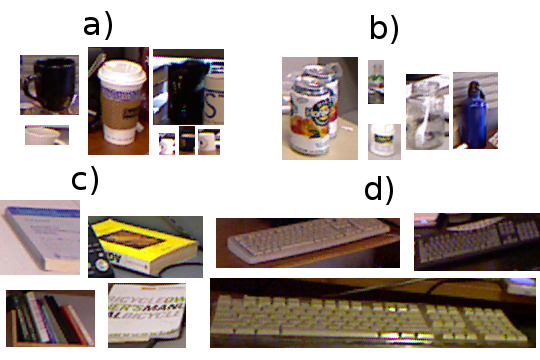
\includegraphics[width=.75\textwidth]{../figs/b3do_objects}
    \caption{B3DO objects: a) cups b) bottles c) books d) keyboards}
    \label{fig:b3do_objects}
    \end{figure}    
    
    The Berkeley 3D Object dataset, shown in \refFig{fig:b3do_objects}, was specifically designed for the purpose of object detection and classification. It consists of cluttered images in indoor environment, with many labelled and random objects per image. The images are often poorly lit and objects are partially occluded. There are around 50 classes with more than 20 examples in each of them. RGBD data are provided as pairs of colour images (8 bit RGB jpeg files) and depth maps (16 bit png files). Images are densely labelled --- for every pair of images there is an xml file with annotations. Each annotation states a category of an object as well as it's bounding box location. Since neither image segmentation nor object detection is addressed in this paper we had to extract objects from the images before the dataset could be used.

  \subsection{The University of Tokyo Dataset}	
    \begin{figure}[!ht]
    \centering
    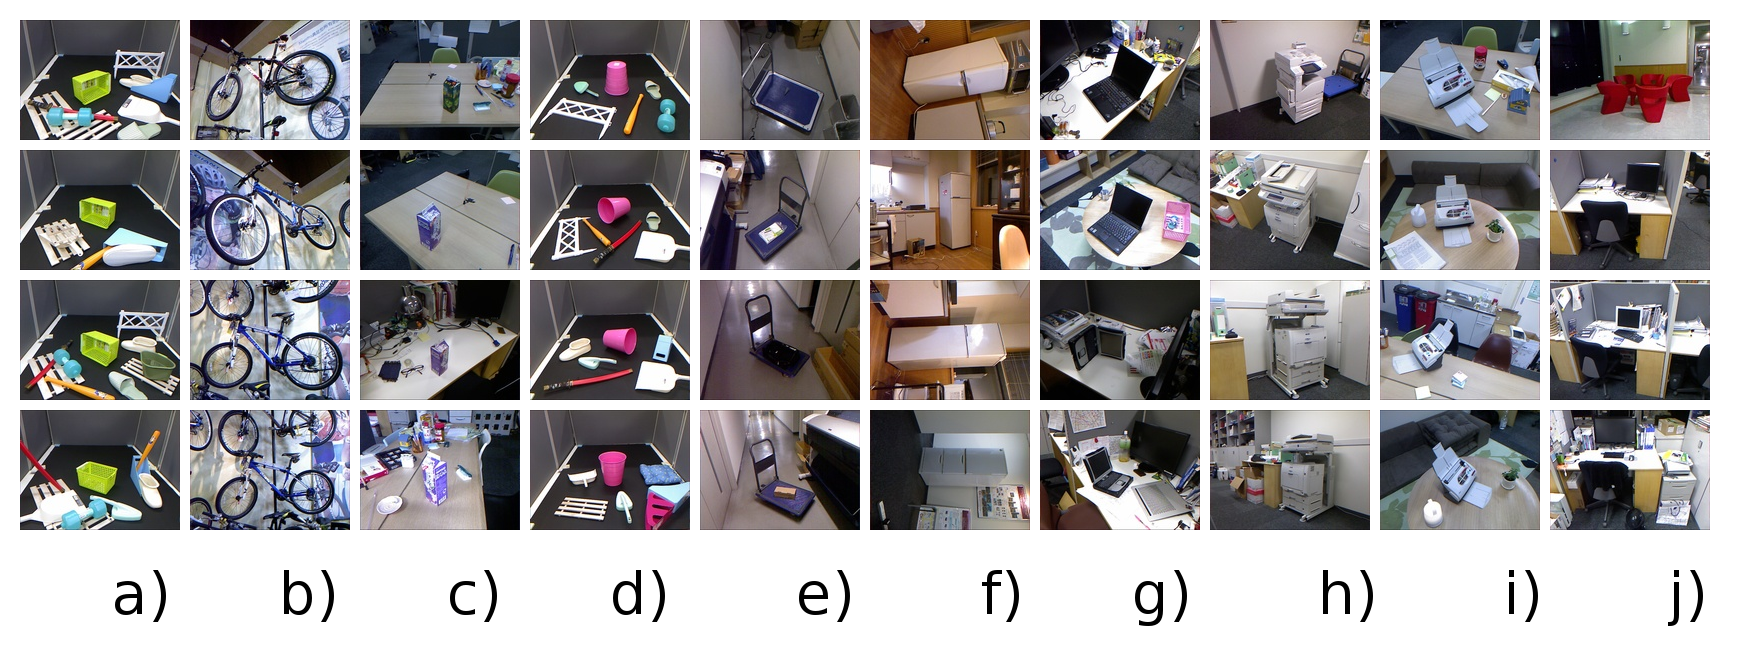
\includegraphics[width=1\textwidth]{../figs/tokyo_horizontal}
    \caption{The Tokyo dataset: a) basket b) bicycle c) box d) bucket e) cart f) freezer g) notebook h) printer i) scanner j) scene}
    \label{fig:tokyo}
    \end{figure}

    The Tokyo dataset, shown in \refFig{fig:tokyo}, is comprised of high quality images of single labelled objects in different settings, with changing viewpoint, object orientation and texture. Additional unlabelled object can be present, however, and should not be taken into account. No bounding boxes are given, which renders the classification task similar to the scene classification problem. The dataset is presented as colour images (8 bit RGB jpeg files) and depth maps (csv files with XYZ coordinates of each pixel). This dataset is aimed at the task of object classification in casual images.

\section{ EXPERIMENTS }
  There is a plenty of algorithms suitable for any of the four steps of Bag of Words image processing. Most of them have multiple tunable parameters and their performance might be interdependent on each other. Comprehensive evaluation is inevitable if an optimal combination is to be selected. Considering the PointCloud Library\footnote{\url{http://pointclouds.org/}} (PCL) alone yields far too many options to test, with 12 keypoint detectors and more than 20 feature descriptors. A literature review helped to narrow the scope of evaluation considerably. All experiments were run on a notebook with Intel Core i7 quad core 2.2 GHz CPU, 8 GB of RAM and a nVidia M540 GPU. 

  \subsection{Detectors and descriptors}
    Keypoint detection algorithms were compared with respect to repeatability and invariance in \cite{pcl_keypoint_comparision} as well as in terms of object retrieval and recognition in \cite{3d_keypoint_eval}. 3D-SIFT and ISS both achieve the highest robustness, while the latter appears to be the best choice for object retrieval. Dense detector (or uniform sampling) achieves the best performance in 2D image classification \cite{tsai2012bag}. Therefore, this paper compares SIFT, ISS and Uniform Sampling keypoint detection techniques. Additionally, PCL descriptors were evaluated in terms of object retrieval performance in \cite{pcl_features}. PFHRGB and SHOTCOLOR delivered the best results, while their simpler counterparts (PFH, FPFH, SHOT) were only a little worse. USC, which is a global descriptor and thus not suitable for the Bag of Words approach, achieved very similar accuracy. The family of PFH descriptors is evaluated in this paper.
    
    \begin{table}[!hbtp]
    \centering
      \caption{Highest accuracy obtained with FPFH, PFH and PFHRGB descriptors on the B3DO dataset}
      \label{tab:desc_b3do}
     \begin{tabular}{*4c}
     \toprule
       Detector & ISS3D & SIFT & Uniform Sampling  \\ 
       Descriptor & \multicolumn{3}{c}{Accuracy {[\%]}} \\
     \midrule
       FPFH & 65.22 &  56.52 & 56.07  \\ 
       PFH & 59.32 &  54.83 & 59.50 \\
       PFHRGB & 63.35 & 52.34 & 53.27 \\
       
   \bottomrule
    \end{tabular}
    \end{table}

    The best results of each detector/descriptor combination on the B3DO dataset are shown in table \ref{tab:desc_b3do}. ISS consistently proved to be the most successful detection algorithm in this setting. SIFT and Uniform Sampling scored similar accuracy but the latter is significantly faster. SIFT is in fact the slowest of the three. As for the descriptors, FPFH delivered the best performance, even though it is an approximate and theoretically the least precise algorithm. It is also the fastest of the three. The combination of ISS and FPFH delivers outstanding results at the lowest computational cost. It allows near real time point-cloud processing and classification. PFHRGB and SIFT are several times slower.
      
  \subsection{Codebook}
    KMeans is used in almost every implementation of the Bag of Words image processing pipeline \cite{tsai2012bag, toldo2009bag}. Csurka \emph{et al} showed that the number of visual words has a significant impact on the final results \cite{csurka2004visual}. A number of tests were run to discover an optimal codebook size for the current setting.

    \begin{figure}[!ht]
    \centering	
    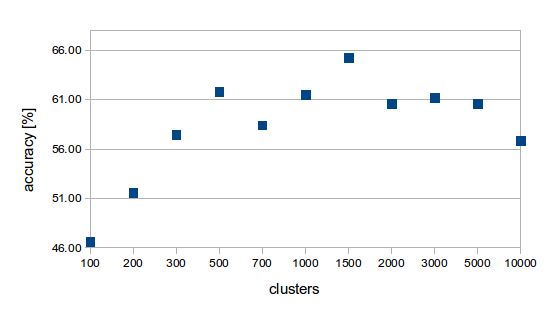
\includegraphics[width=.75\textwidth]{../figs/clustering_centroids_b3do}
    \caption{Influence of dictionary size on the overall accuracy. B3DO dataset with ISS keypoint detector and FPFH feature descriptor}
    \label{fig:cluster_b3do}
    \end{figure}

    The results from \refFig{fig:cluster_b3do} partially confirm Csurka's findings. The performance raises with the increasing number of centroids up to the point of 1500 centroids and 65.22\%. The discrepancies might be caused by the following factors: (1) ISS detector finds too many or irrelevant points, thus introducing noise or (2) The FPFH descriptor has too few dimensions (33) to be divided into more than 1500 regions in a meaningful way. 


  \subsection{B3DO}
    Extracting objects from the B3DO datasets yielded far too many and unbalanced categories. The number of objects in each category varies from 1 (tape) to 299 (table). 8 categories were picked at random with a restriction that there should be at least 50 object instances in a category. Then, the objects were split into train and test set with a proportion of 1:1, which were used for estimation and evaluation respectively.

    The highest accuracy achieved for this dataset is 65.22\%. Table \ref{tab:b3do_conf_matrix} contains a confusion matrix, number of examples per category and accuracy. The confusion matrix depicts classification errors. Let $m_{i, j}$ be an element of the confusion matrix at the $i^{th}$ row and $j^{th}$ column. It shows how many elements from the $i^{th}$ category was assigned to the $j^{th}$ category. A high value of $m_{i, j}$ such that $i \neq j$ indicates that the classifier cannot distinguish those two classes.

    \begin{table}[!ht]
    \centering
    \caption{Results on the B3DO dataset with ISS keypoint detector, FPFH features and a dictionary of 1500 words; \textbf{Average accuracy: 65.22\%}}
    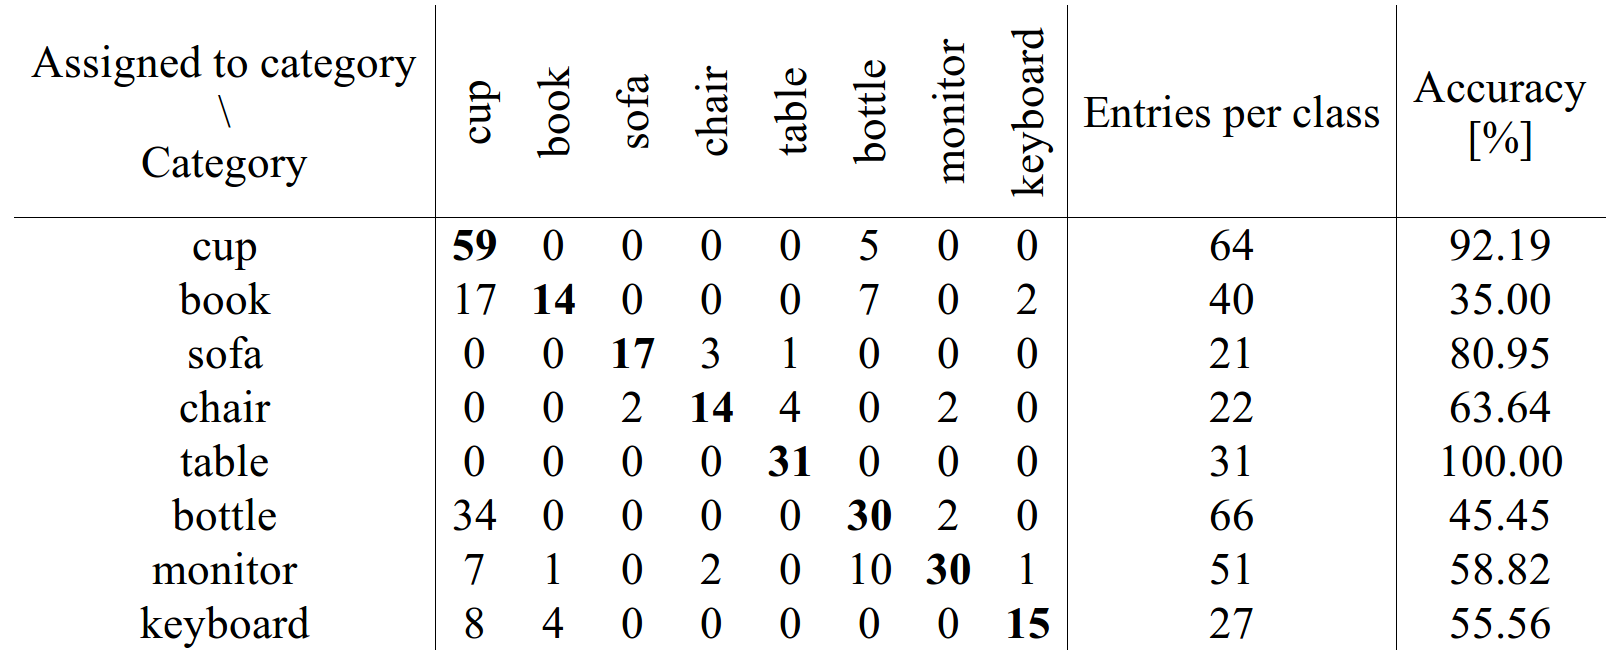
\includegraphics[width=0.9\textwidth]{../figs/b3do_conf_matrix}	
    \label{tab:b3do_conf_matrix}
    \end{table}   

    More than half of the bottles were assigned to the cup category and keyboards were often mistook for books. These two error types are easily explained by a high degree of similarity of objects (bottles and cups are usually round and tall, books and keyboards are flat and rectangular) Surprisingly, however, objects from half of the categories were frequently marked as cups. Some of these misclassification errors might be caused by very poor quality of images. Many of them are occluded poorly lit low resolution images.	

  \subsection{Tokyo}
    \begin{table}[!ht]
    \centering
    \caption{Results on the Tokyo dataset with ISS keypoint detector, PFH features and a dictionary of 3000 words; \textbf{Average accuracy: 62.30\%}}
    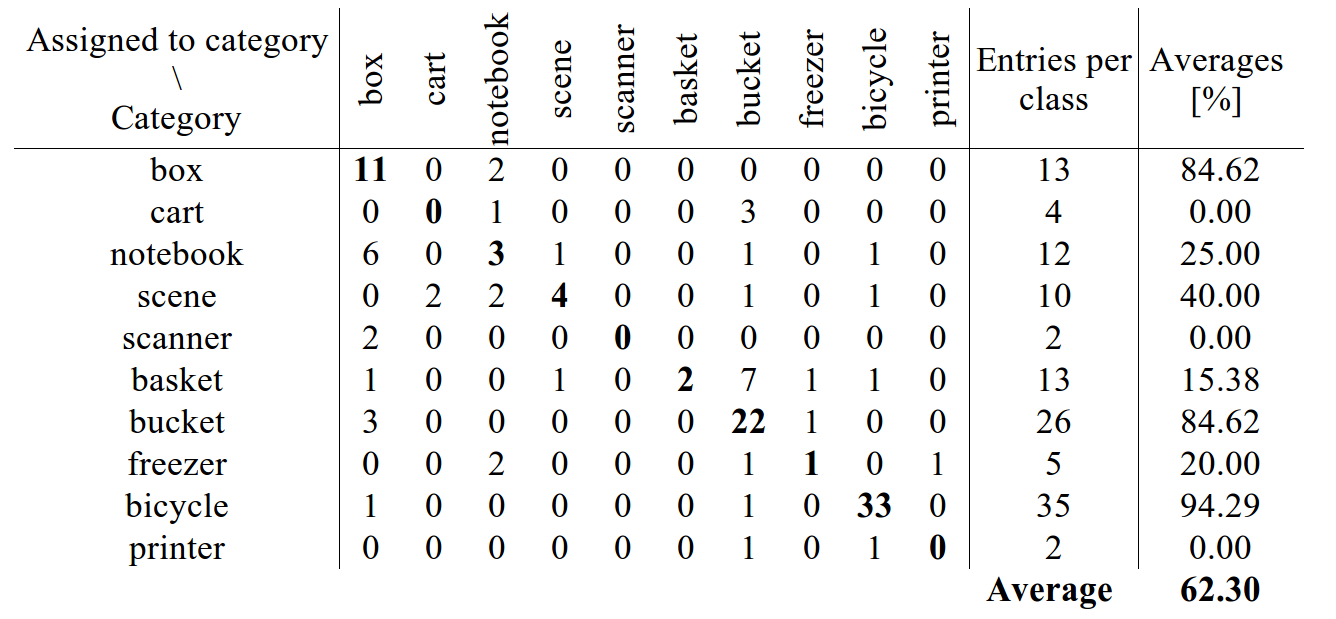
\includegraphics[width=1\textwidth]{../figs/tokyo_conf_matrix}	
    \label{tab:tokyo_conf_matrix}
    \end{table}

    Everyone of the 343 images from the Tokyo dataset were used. Data were split into test and train set in proportions 1:2 in order to provide more training examples due to very limited numbers of objects in some classes. Even tough the overall accuracy achieved on the Tokyo dataset is similar in value to that of the B3DO's, the structure of the result is very different as shown in table \ref{tab:tokyo_conf_matrix}. It is clearly visible that there is a strong correlation between a per class accuracy and the number of entries in this class. The highest performance in the bicycle category is coupled with the largest number of entries. On the other end of the scale there are the printer, scanner and cart categories with 2, 2 and 4 entries respectively and 0\% classification accuracy. On top of that, the differences between some classes are marginal. The majority of carts and baskets were put into the bucket category. It does not surprise, for they are simply akin as can be seen in \refFig{fig:tokyo}.

\section{ CONCLUSION }

  In this paper the issue of three dimensional point cloud classification with a bag of words-based approach was tackled. Two scientific databases suitable for the task of point cloud classification were identified and adapted for the purpose of this work. Presence of such datasets is vital --- they act as benchmarks and allow objective comparison of different solutions of the problem. The following problems emerged: (1)~Point cloud processing is computationally expensive and inefficient. Due to the lack of structure in point clouds (\textit{i.e.} no predefined spatial relationships between points) additional calculations have to be performed (\textit{e.g.} finding nearest neighbours requires at least several distance computations). (2)~There are very few and small databases available. Machine learning algorithms have ravenous appetite for labelled data. As the newest findings in the state-of-the-art 2D object classification suggest, an order of tens of thousands of samples is a prerequisite for any satisfactory results. This work had to make do with less than 300 objects in the train sets. (3)~There is very little interest in the scientific community for this particular task. The majority of research is conducted on retrieval of CAD-like objects from mesh databases.
  
  The achieved results the B3DO and Tokyo datasets are respectively $5.21$ and $6.23$ times higher than random rates ($12.5\%$ and $10\%$). This shows that classification of point clouds is feasible and can be performed in what is close to real time on a mainstream notebook. The accuracy can be further enhanced by generalising 2D algorithms to the 3D domain, while the computational time can be reduced by using a GPU for the most computationally expensive parts of the Bag of Words framework. In conclusion, the depth data does not account for a straightforward improvement in classification accuracy. In fact, it is easier to obtain better results on 2D RGB images, because the best algorithms are not converted to the 3D domain and there is substantially more data available for the 2D. 

\bibliography{kkr13}
\end{document}



